\documentclass{article}
\usepackage{tikz}
\usepackage{amssymb}
\usepackage{amsthm}
\usepackage{amsmath}
\usepackage{mathabx}
\usepackage{listings}
\usepackage{bbm}
\usepackage{caption}
\usepackage{natbib}
\usepackage{float}
\usepackage{hyperref}
\usepackage{setspace}
\usepackage[margin = 1 in]{geometry}
\usepackage{tcolorbox}
\usetikzlibrary{patterns,automata,positioning,arrows}
\title{Strategy Free Machine Learning}
\author{-}
\date{\today}
\hbadness=99999

\begin{document}
\newtheorem{thm}{Theorem}
\newtheorem{cor}{Corollary}
\newtheorem{lem}{Lemma}
\newtheorem{prop}{Proposition}
\newtheorem{conj}{Conjecture}
\newtheorem{algo}{Algorithm}
\newtheorem{obs}{Observation}
\newtheorem{clm}{Claim}
\theoremstyle{definition}
\newtheorem{df}{Definition}
\newtheorem{eg}{Example}
\newtheorem{asm}{Assumption}
\newtheorem{cond}{Condition}
\theoremstyle{remark}
\newtheorem{rmk}{Remark}
\maketitle \onehalfspacing \allowdisplaybreaks \raggedbottom


\section{Short Write-Up} 
There are $n $ strategic agents each providing the label of one data point to the principal. The principal is the learner and builds a machine learning model based on the data points provided by the agents. An agent, $i $, has publicly known feature vector, $x^{\left(i\right)}$, and a private discrete label, $y^{\left(i\right)}$. The objective of the agent is to maximize the probability that her data point is labeled correctly by the principal's model, and the agent can choose to report $\hat{y} ^{\left(i\right)}$ to achieve the objective, with the possibility of misreporting $\hat{y} ^{\left(i\right)} \neq  y^{\left(i\right)}$. We say a dataset is incentive incompatible with respect to the learner, described by a parametric model, if at least one of the $n $ agents has the incentive to misreport.
\newline \newline
The following is the diagram showing a dataset that is incentive incompatible with respect to the multi-class logistic regression model. In the dataset, each of the $n  = 18$ agents, $i $, has a two dimensional feature vector and a private label can take on one of three values: "red", "green", or "blue".
\newline \newline
\begin{figure}[H] \centering 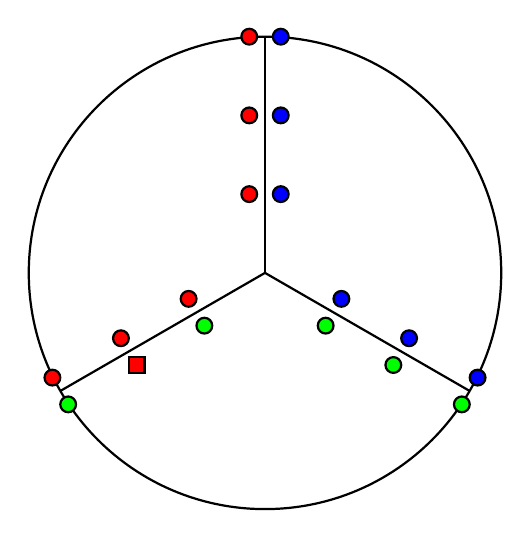
\begin{tikzpicture} [scale = 1] 
\draw[thick] (0.0, 0.0) circle [radius = 3.0];
\draw[thick] (0.0, 0.0) -- (0.0, 3.0);
\draw[fill = blue, thick] (0.2, 1.0) circle [radius = 0.1];
\draw[fill = blue, thick] (0.2, 2.0) circle [radius = 0.1];
\draw[fill = blue, thick] (0.2, 3.0) circle [radius = 0.1];
\draw[fill = red, thick] (-0.2, 1.0) circle [radius = 0.1];
\draw[fill = red, thick] (-0.2, 2.0) circle [radius = 0.1];
\draw[fill = red, thick] (-0.2, 3.0) circle [radius = 0.1];
\draw[thick] (0.0, 0.0) -- (2.6, -1.5);
\draw[fill = blue, thick] (0.97, -0.33) circle [radius = 0.1];
\draw[fill = blue, thick] (1.83, -0.83) circle [radius = 0.1];
\draw[fill = blue, thick] (2.7, -1.33) circle [radius = 0.1];
\draw[fill = green, thick] (0.77, -0.67) circle [radius = 0.1];
\draw[fill = green, thick] (1.63, -1.17) circle [radius = 0.1];
\draw[fill = green, thick] (2.5, -1.67) circle [radius = 0.1];
\draw[thick] (0.0, 0.0) -- (-2.6, -1.5);
\draw[fill = red, thick] (-0.97, -0.33) circle [radius = 0.1];
\draw[fill = red, thick] (-1.83, -0.83) circle [radius = 0.1];
\draw[fill = red, thick] (-2.7, -1.33) circle [radius = 0.1];
\draw[fill = green, thick] (-0.77, -0.67) circle [radius = 0.1];
\draw[fill = red, thick] (-1.73, -1.27) rectangle (-1.53, -1.07);
\draw[fill = green, thick] (-2.5, -1.67) circle [radius = 0.1];
\end{tikzpicture} 
\end{figure}
The $18$ points are located inside a unit circle, and each point is $0.004$ away from the three line segments through the origin that form angles of $120$ degrees between them. There is one point, labeled by a square in the plot, that is on the "incorrect" side of the boundary. Suppose the point corresponds to the feature vector of an agent $i $ with private label "red", then truthfully reporting her label will lead to a multi-class logistic regression model that classifies her point as "green". The probability that this model classifies her point as "red" is $0.3290$. However, if the agent misreports her label as "blue", the resulting model classifies her point as "red" with probability $0.4966$. Therefore, by lying about her label, the agent is able to make the principal learn an incorrect model that classifies her point correctly and with a higher probability.
\newline \newline
The same dataset is also incentive incompatible with respect to the one-vs-rest linear support vector machine if the margin is used as the class "probabilities". However, in this case, the agent, with feature vector corresponding to the blue point close to the center and close to the green point, can only improve the margin slightly without making the model switch from classifying her point incorrectly to classifying her point correctly.
\newline \newline
However, this dataset is incentive compatible with respect to the Naive Bayes classifiers, and in general, there does not exist any dataset that is incentive incompatible with respect to discrete-valued Naive Bayes classifiers. Misreporting will always lead to lower posterior probability of the agent's true label. In addition, no dataset is incentive incompatible with respect to classifiers that minimizes empirical risk with zero-one loss.
\newline \newline

\end{document}
